%%%%%%%%%%%%%%%%%%%%%%%%%%%%%%%%%
\section{Interfaces}
\label{sec:dp-tpcelec-intfc}

The \dual electronics system interfaces to several other systems, starting with the \dword{crp} and the \dword{pd} systems.  The digitized data must in turn flow to the \dword{daq} via the optical links in each \dword{utca} crate. The \dwords{sftchimney} integrate into the cryostat structure and connect to the cryogenics and gas systems. The slow-control system takes on management of the low-voltage power supplies for the \dword{fe} analog electronics and \dword{utca} crates, and  monitors various sensors in the \dwords{sftchimney}. Table~\ref{tab:dp-tpcelec-interfaces} provides the references to the relevant interface documents for each interface, stored in the DUNE document database (DocDB).

\begin{dunetable}
[TPC Electronics System Interface Links]
{p{0.25\textwidth}p{0.5\textwidth}l}
{tab:dp-tpcelec-interfaces}
{TPC Electronics System Interface Links}
Interfacing System & Description & Linked Reference \\ \toprowrule
\dword{crp} & signals from charge collection strips & \citedocdb{6751} \\ \colhline
\dword{pd} & signals from light detection sensors & \citedocdb{6772} \\ \colhline
\dword{daq} & transmission of digitized \dword{cro} and \dword{lro} data & \citedocdb{6778} \\ \colhline
\dword{cisc} & \dword{sftchimney} sensors, control of low-voltage power supplies for \dword{fe} cards, monitoring of \dword{utca} crates & \citedocdb{6784} \\ \colhline
Underground installation & transport of material and underground installation procedure & \citedocdb{7009} \\ \colhline
Integration facility  & logistics and use of integration facility & \citedocdb{7036} \\ \colhline
Calibration & calibration database format & \citedocdb{7063} \\ \colhline
DUNE physics & simulation of the electronics system & \citedocdb{7090} \\ \colhline
Software and computing & reconstruction and analysis tools for charge and light signals & \citedocdb{7117} \\ 
\end{dunetable}

%%%%%%%%%%%%%%%%%%%%%%%%%%%%%%%%%
\subsection{Electronics System to \dword{crp} and Photon Detection Systems}
\label{ssec:dp-tpcelec-intfc-crppmt}

The cold \fdth flange of the \dwords{sftchimney} forms the interface between the \dword{crp} and the \dword{cro} electronics system. On the side facing the cryostat the flange PCB has \num{20} \num{68}\,pin connectors (KEL 8930E-068-178MS-F\footnote{KEL Corporation\texttrademark{}, \url{https://www.kel.jp/english/product/product_detail/?id=490\&pageID=3\%20}.}) for plugging the flat cables from the \dword{crp}. These are \num{68}\,channel twisted-pair flat cables, each carrying signals from \num{32} anode strips and are within the scope of the \dword{crp} system. Each analog \dword{fe} card reads \num{64} anode strips, i.e., signals from two KEL connectors. The order in which the cables are connected to the cold flange determines the mapping of the electronic channels to the physical location of the strips on the \dword{crp} and is coordinated carefully with the \dword{crp} consortium. Figure~\ref{fig:dp-tpcelec-sft-cold-flange} shows two images of the cold \fdth from the \dword{wa105}.

\begin{dunefigure}[Images of the \dword{wa105} \dword{sft} cold \fdth]{fig:dp-tpcelec-sft-cold-flange}
{Images of the \dword{wa105} \dword{sft} cold \fdth with the \dword{fe} cards inserted (right) and signal cables from \dword{crp} connected (left). The \dword{wa105} \dwords{sftchimney} read only \num{320} channels thus requiring \num{5} \dword{fe} cards.}
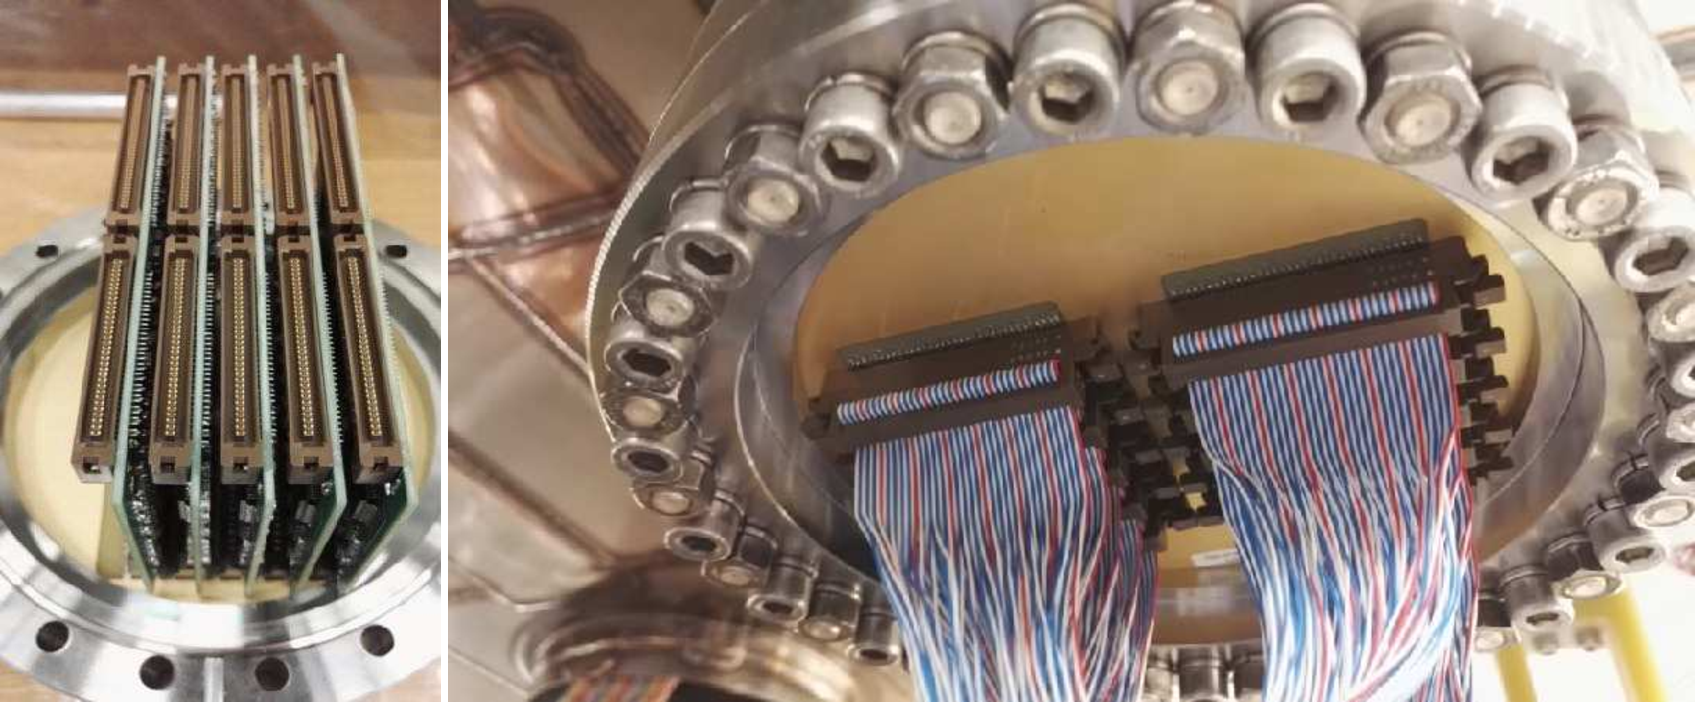
\includegraphics[width=0.8\textwidth]{dp-tpcelec-sft-cold-flange}
\end{dunefigure}

The \dword{lro} electronics system is connected to the specific \dword{lro} signal \fdth flanges on top of the cryostat via coaxial cables, which are within the scope of the \dword{pds}.
The \dword{lro} electronics is designed for negative polarity \dword{pmt} signals, with the amplitude of single \phel{}s on the input of the card between \num{1} and \SI{10}{\milli\volt}. Assuming a typical \dword{pmt} gain of \num{1E6} (not accounting for attenuation of the signals), the Catiroc \dword{asic} can measure a range of \num{1} to \num{400} \phel{}s (\SI{160}{\femto\coulomb} to \SI{70}{\pico\coulomb}). The \dword{adc} samples from \SI{1}{\milli\volt} to \SI{1}{\volt} corresponding to \num{1} to \num{1000} \phel{}s, including the time response of the scintillator the range can increase to $\sim$\num{6000}. Increasing the gain of the \dword{pmt} to \num{1E7}, lowers the upper values by a factor of 10. The internal noise level of the \dword{catiroc} is below \SI{0.1}{\milli\volt}. The objective for the noise level of the \dword{adc} is for each channel to have the \rms noise level greater than \SI{0.5}{LSB}, aiming for \SI{1}{LSB} \SI{0.1}{\milli\volt}.


%%%%%%%%%%%%%%%%%%%%%%%%%%%%%%%%%
\subsection{Electronics System to DAQ System}
\label{ssec:dp-tpcelec-intfc-daq}

The hardware interface between the \dual \dword{cro} and \dword{lro} electronics sub-systems and \dword{daq} has two components. The first interface is the \SI{10}{Gbit/s} optical fibers for data transfer between the \dword{utca} crates and the network interface of the \dword{daq} system. The second one is a \SI{1}{Gbit/s} optical fiber that connects the \dword{daq} \dword{wrgm} switch to the \dual electronics timing system.   

In the current design a given \dword{dpmod} would have \num{245} \SI{10}{Gbit/s} optical links for streaming the digitized data to the \dword{daq} from the \dword{cro} (\num{240} links) and \dword{lro} (\num{5} links) electronics housed in \dword{utca} crates on top of the cryostat structure.  In the current specifications, the fibers are multimode OM3 fibers \cite{om3fibers} with LC-LC connectors suitable for the transmission over distances of up to \SI{300}{\metre}.  They are provided by the \dword{daq} consortium. On the side of the \dword{utca} crate, the fibers are connected to an optical transceiver in the \dword{mch} (two SFP+XAUI links) \cite{natmch}.  On the \dword{daq}, they go to the level-1 machines of the trigger farm, or switches, depending on the network topology adopted in the \dword{daq} system design.

The \SI{1}{Gbit/s} link going from the \dword{wrgm} to the \dual electronics time distribution network serves to provide the synchronization to the reference clock common for the entire FD and derived from a GPSDO clock unit installed on the surface. The clock information is distributed to the \dword{wrmch} slave module in each \dword{utca} crate via a set of \dword{wr} switches. These switches and the interconnecting \SI{1}{Gbit/s} fibers form the timing sub-system of the \dual electronics system and are included in the design of the latter. The \dword{wr} synchronization protocol includes the automatic and continuous calibration of the propagation delays between the master and the connected slaves. This allows maintaining the overall synchronization between different nodes at sub-ns level. The \dword{wrgm} will be located either:
\begin{itemize}
\item{On the surface near the GPSDO. In this case, a single fiber connects it to the \dual timing system underground. The system automatically accounts for the incurred latency due to the extensive fiber length.}
\item{Underground in the \dword{cuc}. In this case, calibration of the propagation delays between GPSDO and the \dword{wrgm} is performed manually, and a timing correction is applied to the data afterward.}
\end{itemize} 

The TPC electronics design assumes that the data are streamed continuously via the \SI{10}{Gbit/s} links to the \dword{daq}, where they are buffered until a trigger decision is made. The triggers are to be issued by processing the buffered data in some suitable sliding time window on the trigger farm machines. The window may be as long as \SI{10}{s} for \dword{snb}-triggered events. The triggers determine whether the data contained in the buffers are to be written on disk. 

The software interface between the \dword{daq} and the electronics system includes the tools for handling the data transmission and buffering, i.e.,  data formatting in \dword{udp} packets, compression and decompression, and exchange of the control packets.

%%%%%%%%%%%%%%%%%%%%%%%%%%%%%%%%%
\subsection{Electronics System to Cryostat and Cryogenics}
\label{ssec:dp-tpcelec-intfc-cryo}

The interface point between the cryostat and the \dual electronics system is at the cryostat penetrations where the \dwords{sftchimney} are installed. Each penetration accommodates the chimney (of external diameter \SI{254}{\mm}). Each chimney has a CF-273 flange welded to its outer structure (see Figure~\ref{fig:dp-tpcelec-sft-chimney-crosspipe}). After the chimney is inserted, this flange is in contact with the corresponding flange on the crossing (or penetration) pipe embedded in the cryostat structure to which it is eventually fastened. In order to avoid any leaks at this interface a CF-273 copper gasket is used to ensure the vacuum tightness.  

\fixme{it would be nice to replace this figure with an image from the actual cryostat 3D model if such exists}
\begin{dunefigure}[Details of \dword{sftchimney} interface to the cryostat structure]{fig:dp-tpcelec-sft-chimney-crosspipe}
{Details of \dword{sftchimney} interface to the cryostat structure.}
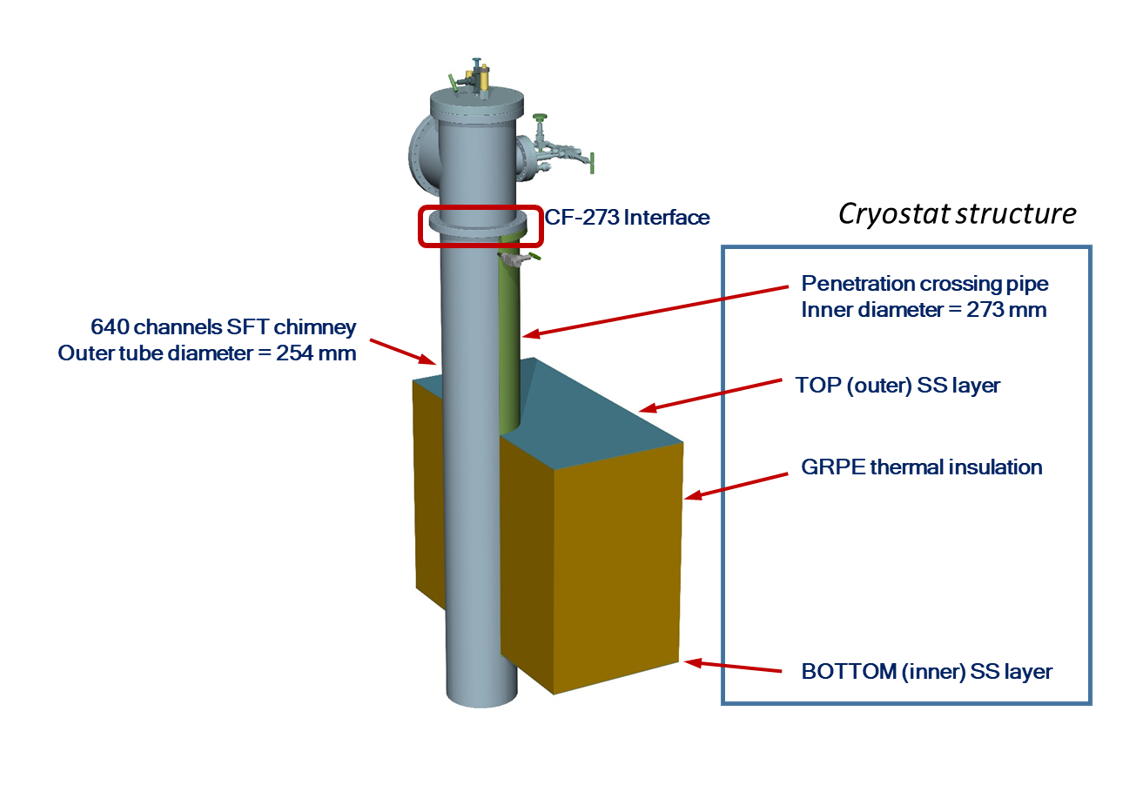
\includegraphics[width=0.7\textwidth]{dp-tpcelec-sft-chimney-crosspipe}
\end{dunefigure}

Each chimney contains a heat exchanger copper coil cooled with \lar. There are two (inlet and outlet) stainless steel pipe connections with \SI{10}{\mm} and \SI{12}{\mm} inner and outer diameters, respectively, that need to be branched to the respective system for the \lar delivery and recirculation. In addition, a connection for nitrogen gas line with the same pipe dimensions as those for the \lar cooling, is used for filling the chimney after it is closed following the installation of the \dword{fe} electronics. The nitrogen line is also required for flushing the chimney in the case of an access to the \dword{fe} cards after the \dword{dpmod} is cooled for the operation. 

The \dword{utca} crates for charge readout are installed within a short \SI{<0.5}{\meter} distance from the \dwords{sftchimney} on top of the cryostat roof. The five \dword{utca} crates for the light readout are also placed on the roof of the cryostat at optimal locations defined by the routing of the \dword{pmt} signal cables. The required volume to accommodate the crates is roughly \SI[product-units=power]{60x50x40}{\cm}. 

%%%%%%%%%%%%%%%%%%%%%%%%%%%%%%%%%
\subsection{Electronics System to Slow Control System}
\label{ssec:dp-tpcelec-intfc-sc}

The integration with the slow control of the low-voltage power supply system for the \dword{fe} cards and \dword{utca} crates is required to enable the remote management and monitoring (current consumption by \dwords{asic}, set voltage, etc.). In addition, the \dwords{sftchimney} contain several sensors that need to be monitored. These include a pressure transducer that measures the pressure inside the chimney and at least two temperature probes (PT1000) that monitor the gas temperature inside near the cold flange at the bottom and close to the warm flange at the top. The readout of the \dword{utca} crate information and the sensors in the \dwords{sftchimney} is part of the Slow Control system.
